\chapter{Introduction}\label{sec:introduction}

SOME MORE GENERAL INTRO TEXT HERE?

The ability to understand spoken language, to recognize faces and to distinguish types of fruit comes naturally to humans, even though these processes of pattern recognition and classification are inherently complex. Machine learning (ML), a subtopic of artificial intelligence, is concerned with the development of algorithms that perform these types of tasks, thus enabling computers to find and recognise patterns in data and classify unknown inputs based on previous training with labelled inputs. Such algorithms make the core of e.g. human speech recognition and recommendation engines as used by Amazon.
% and algorithms that can predict heart disease from real-time electrocardiograms \citep{acharya2015integrated, pazzani2007content}.

According to \cite{bigdata}, approximately 2.5 quintillion (${10}^{18}$) bytes of digital data are created every day. This growing number implies that every area dealing with data will eventually require advanced algorithms that can make sense of data content, retrieve patterns and reveal correlations. However, most ML algorithms involve the execution of computationally expensive operations and doing so on large data sets inevitably takes a lot of time \cite{bekkerman2011scaling}. Thus, it becomes increasingly important to find efficient ways of dealing with big data.
%and/or reduce the computational complexity of the algorithms.

A promising solution is the use of quantum computation which has been researched intensively in the last few decades. Quantum computers (QCs) use quantum mechanical systems and their special properties to manipulate and process information in ways that are impossible to implement on classical computers. The quantum equivalent to a classical bit is called a quantum bit (qubit) and additionally to being in either state \0 or \1 it can be in their linear superposition.

%\begin{equation}
%\label{equ: simplequbit}
%\ket{q} = \alpha \ket{0} + \beta \ket{1}
%\end{equation}
%where $\alpha$ and $\beta$ are complex numbers and often referred to as amplitudes. When measuring qubit $\ket{q}$ it will take the value \0 with a probability of ${|\alpha|}^{2}$ and \1 with a probability of ${|\beta|}^{2}$. Since the total probability has to sum to unity, the normalization condition ${|\alpha|}^{2} + {|\beta|}^{2} =  1$ must be satisfied at all times.

This peculiar property gives rise to so-called quantum parallelism, which enables the execution of certain operations on many quantum states at the same time. Despite this advantage, the difficulty in quantum computation lies in the retrieval of the computed solution since a measurement of a qubit collapses it into a single classical bit and thereby destroys information about its previous superposition. Several quantum algorithms have been proposed that provide exponential speed-ups when compared to their classical counterparts with Shor's prime factorization algorithm being the most famous \cite{shor1994}.
%As another example, Grover's quantum database search algorithm enables finding a single element in a list of $N$ elements within roughly $\sqrt{N}$ quantum mechanical steps instead of $N$ classical steps \citep{grover}.
Hence, quantum computation has the potential to vastly improve computational power, speed up the processing of big data and solve certain problems that are practically unsolvable on classical computers. 

%for the QML toolbox to be complete a quantum algorithm to solve systems of linear equations is needed since most ML algorithms rely on solving those.

Considering these advantages, the combination of quantum computation and classical ML into the new field of quantum machine learning (QML) seems almost natural. There are currently two main ideas on how to merge quantum computation with ML, namely a) running the classical algorithm on a classical computer and outsourcing only the computationally intensive task to a QC or b) executing the quantum version of the entire algorithm on a QC. Current QML research mostly focusses on the latter approach by developing quantum algorithms that tap into the full potential of quantum parallelism.

\section{Motivation}
\label{sec:motivation}

Classical ML is a very practical topic since it can be directly tested, verified and implemented on any commercial classical computer. So far, QML has been of almost entirely theoretical nature since the required computational resources are not in place yet. To yield reliable solutions QML algorithms often require a relatively large number of error-corrected qubits and some sort of quantum data storage such as the proposed quantum random access memory (qRAM) \cite{qRAM}. However, to date the maximum number of superconducting qubits reportedly used for calculation is nine, the D-Wave II quantum annealing device delivers 1152 qubits but can only solve a narrow class of problems and a qRAM has not been developed yet \cite{hydrogensimulation, dwave2}. Furthermore, qubit error-correction is still a very active research field and most of the described preliminary QCs deal with non error-corrected qubits with short lifetimes and are, thus, impractical for large QML implementations.

Until now there have been only few experimental verifications of QML algorithms that establish proof-of-concept. \cite{Li2015} successfully distinguished a handwritten six from a nine using a quantum support vector machine on a four-qubit nuclear magnetic resonance test bench. In addition, \cite{Cai2015} were first to experimentally demonstrate quantum machine learning on a photonic QC and showed that the distance between two vectors and their inner product can indeed be computed quantum mechanically. Lastly, \cite{Riste2015} solved a learning parity problem with five superconducting qubits and found that a quantum advantage can already be observed in non error-corrected systems.

%Consequently,
Considering the gap between the number of proposed QML algorithms and the few experimental realisations, it remains important to find QML problems which can already be implemented on small-scale QCs. Hence, the purpose of this study is to provide proof-of-concept implementation of selected QML algorithms on small datasets. This is an important step in the attempt to shift QML from a purely theoretical research area to a more applied field such as classical ML. 

\section{Research Question}
\label{sec:researchquestion}


Don't know where this should go!

Matthias Troyer citation for this part:

There are many different ways of realising a QC such as using trapped ions, single photon sources or superconducting Josephon junctions, etc. Depending on the chosen substrate, different sets of quantum logic gates can be implemented and in order to run a quantum algorithm  it has to be mapped to the available hardware. Thus, quantum algorithms have to be translated (compiled) into a series of gates consisting only of quantum gates from the available gate set. This is referred to as \emph{quantum compilation}.

Finding optimal ways of compiling a given quantum algorithm as well as designing a high-level programming language or environment similar to that of classical computer code editors is called \emph{quantum software engineering}.


In light of the theoretical nature of current QML research and the small number of experimental realizations, this research will address the following question:

%NARROW DOWN THE RESEARCH QUESTION!
\centering\textbf{How can a theoretically proposed k-nearest neighbour quantum machine learning algorithm be implemented on small-scale quantum computers?}

%Alternatives:
%Is it possible to experimentally demonstrate that two QML algorithms proposed by \cite{Schuld2014, Schuld2016} can already solve a small ML problem using classical simulation or IBMs quantum processor?
%Is it possible to already implement and solve a small ML problem on IBMs publicly available quantum computer?

\justify
The following sections will outline the steps required and the tools used in order to answer this research question. 

\chapter{Theoretical Foundations}\label{sec:theory}

CHECK FOOTNOTE NUMBERS IN WHOLE DOCUMENT!
\section{Quantum Bits}
\label{subsec:qubits}

\subsection{Single Qubit Systems}
\label{subsubsec:qubits}
%Classical computers manipulate bits and the quantum equivalent is called a quantum bit, often abbreviated as qubit.
Classical computers manipulate bits, whereas quantum computer's most fundamental unit is called a quantum bit, often abbreviated as qubit. Bits as well as qubits are binary entities, meaning they can only take the values 0 and 1.

A good example for a physical implementation of a qubit is the single electron of a hydrogen atom sketched in Fig.~\ref{img:qubitatom}. Usually, the electron is found in its ground state which one can define as the \0 state of the qubit. Using a laser pulse the electron can be excited into the next highest valence shell which one can define as the \1 state of the qubit. After some time $t$ the electron will decohere to its ground state (\0) which is called the longitudinal coherence or amplitude damping time and is an important parameter for measuring qubit lifetimes.

\begin{figure}[!ht]
       \centering
       \includegraphics[width=0.9\textwidth]{img/qubitimplementation.jpeg}
       \caption{\label{fig:qubitatom} A simple example of a physical qubit using the electron of a hydrogen atom}
\end{figure}

\footnotetext[1]{Reprinted from RF Wireless World, n.d., Retrieved December 23, 2016, from \url{http://www.rfwireless-world.com/Terminology/Difference-between-Bit-and-Qubit.html}. Copyright 2012 by RF Wireless World. Reprinted with permission.}

A classical non-probabilistic bit can only be in one of the two possible states at once. In contrast, qubits obey the laws of quantum mechanics, which gives rise to the powerful property that - besides being a definite 0 or 1 - they can also be in a superposition of the two states. Mathematically this is expressed as a linear combination of the states 0 and 1:

\begin{equation}
\label{equ: simplequbit}
\ket{\psi} = \alpha \ket{0} + \beta \ket{1}
\end{equation}

where $\alpha$ and $\beta$ are complex coefficients ($\alpha, \beta \in \mathbb{C}$) and are often referred to as phase factors or amplitudes. \0 is the Dirac notation for the qubit being in state 0 and it represents a two-dimensional vector in a complex 2-D vector space (called Hilbert space $\mathcal{H}_{2}$). \0 and \1 are the computational basis states and they constitute an orthonormal basis of $\mathcal{H}_{2}$. For the sake of clarity, \0 and \1 can be thought of as the 2-D vectors shown below.

APPROXIMATELY EQUAL SIGN!
\begin{equation}
\label{equ: 0and1kets}
\ket{0} =  \colvec{1\\0} \quad \quad \ket{1} = \colvec{0\\1}
\end{equation}

Subbing these vectors into Equ.~\ref{equ: simplequbit} yields the vector representation of $\ket{\psi}$:
\begin{equation}
\label{equ: simplequbitvector}
\ket{\psi} = \alpha \colvec{1\\0} + \beta \colvec{0\\1} = \colvec{\alpha\\\beta}
\end{equation}

In the cases $\alpha = 1$ or $\beta = 1$ there is no quantum behaviour since the qubit is not in a superposition. However, if for example $\alpha = \beta = \frac{1}{\sqrt{2}}$ the qubit is in an equal quantum superposition which is impossible to achieve with a classical computer. This leads to another important qubit lifetime parameter - the transversal coherence or phase damping time. It is measured by preparing the equal superposition $\frac{\ket{0}+\ket{1}}{\sqrt{2}}$ and due to unavoidable interaction with the environment after some time $t$ the quantum behaviour will be lost and the state will either be a definite \0 or \1. The process of losing quantum behaviour is called \emph{decoherence}.

However, even though a qubit can be in a superposition of \0 and \1, when measured it will take the value \0 with a probability of
\begin{equation}
\label{equ:bornrule0}
Prob(\ket{0}) = {|\alpha|}^{2}
\end{equation}
and \1 with a probability of 
\begin{equation}
\label{equ:bornrule1}
Prob(\ket{1}) = {|\beta|}^{2}
\end{equation}

The fact that the probability of measuring a particular state is equal the absolute value squared of the respective amplitude is called Born rule (citation). Since the total probability of measuring any value has to be 1, the following normalization condition must be satisfied:
\begin{equation}
\label{equ: normalization}
{|\alpha|}^{2} + {|\beta|}^{2} =  1
\end{equation}
Therefore, a qubit is inherently probabilistic but when measured it collapses into a single classical bit (0 or 1). It follows that a measurement destroys information about the superposition of the qubit (the values of $\alpha$ and $\beta$). This constitutes one of the main difficulties when designing quantum algorithms since only limited information can be obtained about the final states of the qubits in the quantum computer.

Similar to logic gates in a classical computer, a QC manipulates qubit by means of quantum logic gates which will be introduced in detail in Section~\ref{subsec:quantumlogicgates}. Generally, an arbitrary quantum logic gate U acting on a single qubit state is a linear transformation given by a 2x2 matrix whose action on $\ket{\psi}$ is defined as:

\begin{equation}
\label{equ:unitarytransformation}
U \ket{\psi} = \begin{pmatrix}
 a & b \\ 
 c & d
 \end{pmatrix} \colvec{\alpha\\\beta} = \colvec{a*\alpha+b*\beta\\c*\alpha+d*\beta}
\end{equation}

Matrix $U$ must be unitary which means that a) its determinant is equal to unity and b) its Hermitian conjugate $U^\dagger$ must be equal to its inverse (see Equ.~\ref{equ:unitarydef1} and ~\ref{equ:unitarydef2}). All quantum logic gates must be unitary since this preserves the normalization of the qubit state it is acting on.

\begin{align}
\label{equ:unitarydef1}
a)& \mid det(U) \mid = 1 \\ 
\label{equ:unitarydef2}
b)& \quad UU^\dagger = U^\dagger U = \mathbb{1} = UU^{-1} = U^{-1}U
\end{align} 

Using spherical polar coordinates, a single qubit can be visualized on the so-called Bloch sphere by parameterising $\alpha$ and $\beta$ in Equ.~\ref{equ: simplequbit} as follows:

\begin{equation}
\label{equ: blochqubit}
\ket{q} = \cos\frac{\theta}{2} \ket{0} + e^{i \phi} \sin\frac{\theta}{2} \ket{1}
\end{equation}

The Bloch sphere has a radius of 1 and is therefore a unit sphere. The \0 qubit state is defined to lie along the positive z-axis ($\hat{z}$) and the \1 state is defined to lie along the negative z-axis ($-\hat{z}$) as labelled in Fig.~\ref{fig:blochsphere}. At this point, it is important to note that these two states are mutually orthogonal in $\mathcal{H}_{2}$ even though they are not orthogonal on the Bloch sphere. 

Qubit states on the Bloch equator such as the $\hat{x}$ and $\hat{y}$ coordinate axes represent equal superpositions where \0 and \1 both have measurement probabilities equal to $0.5$. The $\hat{x}$-axis for example represents the equal superposition $\ket{q} = \frac{1}{\sqrt{2}} \ket{0} + \frac{1}{\sqrt{2}} \ket{1}$. As illustrated in Fig.~\ref{fig:blochsphere} any arbitrary 2-D qubit state $\ket{\psi}$ can be decomposed into the polar angles $\theta$ and $\phi$ and visualized as a vector on the Bloch sphere. Such an object is called the Bloch vector of the qubit state $\ket{\psi}$. The Bloch sphere will be the main visualization tool for qubit manipulations in this thesis.

\begin{figure}[!ht]
       \centering
       \includegraphics[scale=0.07]{img/blochsphere.png}
       \caption{\label{fig:blochsphere} An arbitrary two-dimensional qubit $\ket{\psi}$ visualized on the Bloch sphere.$^{2}$}
\end{figure}

\footnotetext[2]{Reprinted from Wikipedia, n.d., Retrieved September 7, 2016, from \url{https://en.wikipedia.org/wiki/Bloch_Sphere}. Copyright 2012 by Glosser.ca. Reprinted with permission.}

\subsection{Multiple Qubit Systems}
\label{subsec:multiplequbitsystems}

A classical computer with one bit of memory is not particularly useful and equally a QC with one qubit is rather useless. In order to be able to perform large and complicated computations many individual qubits need to be combined to create a large QC. When moving from single to multi qubit systems a new mathematical tool, the so-called tensor product (symbol $\otimes$), is needed. A tensor product of two qubits is written as:

\begin{equation}
\ket{\psi} \otimes \ket{\psi} = \ket{0} \otimes \ket{0} = \ket{00}
\end{equation}
 
whereby the last expression omits the $\otimes$ symbol which is the shorthand form of a tensor product between two qubits.

In vector notation a tensor product of two vectors (\textcolor{red}{red} and \textcolor{green}{green}) is defined as shown below:

\begin{equation}
\label{equ:tensor2qubits}
\ket{\textcolor{red}{0}\textcolor{green}{0}} = \textcolor{red}{\ket{0}} \otimes \textcolor{green}{\ket{0}} = \textcolor{red}{\colvec{1\\0}} \otimes \textcolor{green}{\colvec{1\\0}} = \colvec{\textcolor{red}{1}*\textcolor{green}{\colvec{1\\0}}\\\textcolor{red}{0}*\textcolor{green}{\colvec{1\\0}}} = \colvec{1\\0\\0\\0}
\end{equation}

The last expression in Equ.~\ref{equ:tensor2qubits} shows that the two-qubit state $\ket{00}$ is no longer two but four-dimensional. Hence, it lives in a four-dimensional Hilbert space $\mathcal{H}_{4}$. A quantum gate acting on multiple qubits can therefore not have the same dimensions as a single-qubit gate (Equ.~\ref{equ:unitarytransformation}) which demands for a new gate formalism for multi qubit systems.

Consider wanting to apply an arbitrary single-qubit gate U (Equ.~\ref{equ:unitarytransformation}) to the first qubit and leaving the second qubit unchanged, essentially applying the identity matrix $\mathbb{1}$ to it. To do this, one defines the tensor product of two matrices as follows,

\begin{equation}
\label{equ:matrixtensorproduct}
\textcolor{red}{U} \otimes \textcolor{green}{\mathbb{1}} =\textcolor{red}{\begin{pmatrix}
 a & b \\ 
 c & d
 \end{pmatrix}} \otimes \textcolor{green}{\begin{pmatrix}
 1 & 0 \\ 
 0 & 1
 \end{pmatrix}} = \begin{pmatrix}
 \textcolor{red}{a}*\textcolor{green}{\begin{pmatrix}
 1 & 0 \\ 
 0 & 1
 \end{pmatrix}} & \textcolor{red}{b}*\textcolor{green}{\begin{pmatrix}
 1 & 0 \\ 
 0 & 1
 \end{pmatrix}} \\ 
 \textcolor{red}{c}*\textcolor{green}{\begin{pmatrix}
 1 & 0 \\ 
 0 & 1
 \end{pmatrix}} & \textcolor{red}{d}*\textcolor{green}{\begin{pmatrix}
 1 & 0 \\ 
 0 & 1
 \end{pmatrix}}
 \end{pmatrix} = \begin{pmatrix}
 a & 0 & b & 0 \\ 
 0 & a & 0 & b \\ 
 c & 0 & d & 0 \\ 
 0 & c & 0 & d 
 \end{pmatrix}
\end{equation}

Thus, the result of the tensor product $U \otimes \mathbb{1}$ is a unitary 4x4 matrix which can now be used to linearly transform the 4x1 vector representing the $\ket{00}$ state in Equ.~\ref{equ:tensor2qubits}:

\begin{equation}
\label{equ:2qubitlineartransform1}
U \otimes \mathbb{1} \ket{00} = \begin{pmatrix}
 a & 0 & b & 0 \\ 
 0 & a & 0 & b \\ 
 c & 0 & d & 0 \\ 
 0 & c & 0 & d 
 \end{pmatrix} \colvec{1\\0\\0\\0} = \colvec{a\\0\\c\\0}
\end{equation}

One can also first perform the single qubit operations on the respective qubits followed by the tensor product of the two resulting vectors:

\begin{equation}
\label{equ:2qubitlineartransform2}
(U \otimes \mathbb{1})(\ket{0} \otimes \ket{0})= U\ket{0} \otimes \mathbb{1}\ket{0} = \begin{pmatrix}
 a & b \\ 
 c & d
 \end{pmatrix} \colvec{1\\0} \otimes \begin{pmatrix}
 1 & 0 \\ 
 0 & 1
 \end{pmatrix} \colvec{1\\0} = \colvec{a\\c} \otimes \colvec{1\\0} = \colvec{a\\0\\c\\0}
\end{equation}

This formalism can be extended to any number of qubits and the use of tensor products leads to an exponential increase in the dimensionality of the Hilbert space. Hence, $n$ qubits live in a $2^n$-dimensional Hilbert space ($\mathcal{H}_{2}^\otimes n$) and can store the content of $2^n$ classical bits. As an example, only 33 qubits can store the equivalent of $2^33 = 8,589,934,592$ bits (1 gigabyte) which bears the potential for enourmous speed-ups in computations as will be demonstrated later.

Lastly, when considering multi qubit systems one will find composite states that can or cannot be factorized. Consider for example the last expression in Equ.~\ref{equ:2qubitlineartransform2} which can be reexpressed as follows,

\begin{equation}
\label{equ:2qubitreexpressed}
\colvec{a\\0\\c\\0} = a\colvec{1\\0\\0\\0} + 0\colvec{0\\1\\0\\0} + c \colvec{0\\0\\1\\0} + 0\colvec{0\\0\\0\\1} =  a\ket{00} + 0 \ket{01} + c \ket{10} + 0\ket{11}
\end{equation}

This can be factorized into the following tensor product:

\begin{equation}
\label{equ:2qubitfactorized}
a\ket{00} + c \ket{10} = (a\ket{0} + c \ket{1})\otimes \ket{0}
\end{equation}

In contrast, consider the following state:

\begin{equation}
\label{equ:2qubitnonfactorized}
\ket{\phi} = \frac{\ket{00} + \ket{11}}{\sqrt{2}}
\end{equation}

It is straightforward to see that there is no way to factorize the state $\ket{\phi}$ into a tensor product of two states.
Now imagine, two people Andy and Beatrice are given two electrons prepared in the quantum state $\ket{\phi}$. Andy keeps the first electron in the lab and Beatrice takes the second electron to her house. Andy gets interested in measuring if his electron is in the $\ket{0}$ or $\ket{1}$ state and performs a measurement. He finds the electron to be in the $\ket{1}$ state. From Equ.~\ref{equ:2qubitnonfactorized} and knowing that measurement collapses a superposition the post-measurement (PM) state $\ket{\phi}_{PM}$ is given by:

\begin{equation}
\label{equ:2qubitcollapsed}
\ket{\phi}_{PM} = \ket{11}
\end{equation}

Looking at this expression tells Andy that Beatrice's electron must be in state $\ket{1}$ as well without having measured her electron! Even more suprising is the fact that the second electron was nowhere close to Andy and he was still able to determine its state. 

Non-local correlations between qubit measurement outcomes is a peculiar quantum property of non-factorising quantum states and is called \emph{entanglement}. It is an integral part of quantum computation and Section~\ref{subsubsubsec:cnotgate} will give a concrete example of how to create such a state in a QC.

%%%%% SECTION: Q LOGIC GATES


\section{Quantum Logic Gates}
\label{subsec:quantumlogicgates}
In order to perform quantum computations, tools, analogous to the classical logic gates, are needed for qubit manipulation. Quantum logic gates are square matrices that can be visualized as rotations on the Bloch sphere. The following subsections will introduce the major single and multi qubit logic gates.

\subsection{Single Qubit Gates}
\label{subsubsec:singlequbitgates} 

\subsubsection{Qubit Flip (X) Gate}
\label{subsubsubsec:xgate}

The quantum equivalent of the classical NOT logic gate is called X gate and is given by the 1\textsuperscript{st} Pauli matrix:

\begin{equation}
\sigma_{1} = X = \begin{pmatrix}
 0 & 1 \\ 
 1 & 0
 \end{pmatrix}
\end{equation}


The action of a quantum gate on the arbitrary qubit state $\ket{\psi}$ (Equ.~\ref{equ: simplequbitvector}) can be analysed using the gate's matrix and the qubit's vector representation. Applying some straightforward linear algebra yields:

\begin{equation}
\label{equ:xverification1}
X \otimes \ket{\psi} = X \otimes (\alpha \ket{0} + \beta \ket{1}) = \begin{pmatrix}
 0 & 1 \\ 
 1 & 0
 \end{pmatrix} \begin{pmatrix}
 \alpha  \\ 
 \beta
 \end{pmatrix} = \begin{pmatrix}
 \beta  \\ 
 \alpha
 \end{pmatrix} = \beta \ket{0} + \alpha \ket{1}
\end{equation}

Thus, applying the X gate to qubit state $\ket{\psi}$ swaps the amplitudes of \0 and \1. More specifically, applying X to the \0 state results in the \1 state,

\begin{equation}
\label{equ:xverification2}
X \otimes \ket{0} = \begin{pmatrix}
 0 & 1 \\ 
 1 & 0
 \end{pmatrix} \begin{pmatrix}
 1  \\ 
 0
 \end{pmatrix} = \begin{pmatrix}
 0  \\ 
 1 \end{pmatrix} =  \ket{1}
\end{equation}

In terms of the example with the electron of a hydrogen atom shown in Fig.~\ref{img:qubitatom} an X gate can be implemented by exciting the electron from the ground state ($\ket{0}$) into the next highest electron valence shell ($\ket{1}$) using a controlled laser pulse.

%consider the qubit initially being in state \0. Applying an X gate will flip the qubit into the \1 state which can be implemented in the lab by exciting the electron into the next highest electron valence shell using a controlled laser pulse.

The \0 state is recovered when applying X again to the \1 state,

\begin{equation}
\label{equ:xverification3}
X \otimes \ket{1} = \begin{pmatrix}
 0 & 1 \\ 
 1 & 0
 \end{pmatrix} \begin{pmatrix}
 0  \\ 
 1
 \end{pmatrix} = \begin{pmatrix}
 1  \\ 
 0 \end{pmatrix} =  \ket{0}
\end{equation}

On the Bloch sphere, the X gate corresponds to an anti-clockwise $\pi$ rotation around the x-axis as shown in Fig.~\ref{img:blochxgate}.

\begin{figure}[ht]
   \centering
   \includegraphics[width=0.5\textwidth]{img/blochxgate.png}
   \caption{Visualization of the X gate on the Bloch sphere. Initial state (black) transformed to final state (red).}
   \label{img:blochxgate}
\end{figure}

From Equ.~\ref{equ:xverification1},~\ref{equ:xverification2} and~\ref{equ:xverification3} it follows that X is its own inverse as well as its own Hermitian conjugate:
\begin{align}
XX &= XX^\dagger = \mathbb{1} \\
X &= X^{-1} = X^\dagger
\end{align}

The action, circuit \& matrix representation and Bloch sphere visualization for the most important single-qubit quantum logic gates are summarised in Table~\ref{tab:singlequbitgates}  below.

\begin{table}[H]
\caption{Table of major single-qubit quantum logic gates.}\vspace{1em}
\label{tab:singlequbitgates}
\begin{tabular}{ C{0.3cm}  C{2cm}  C{1.5cm}  C{1.5cm} C{2.5cm} C{2cm} C{3.5cm}}\hline
Gate & Name & Circuit representation & Matrix & Description & Rotation & Bloch sphere \\ \midrule
$\mathbb{1}$ & Identity & \includegraphics[width=0.1\textwidth]{img/identitycircuit.png} & $\begin{pmatrix}
 1 & 0 \\ 
 0 & 1
 \end{pmatrix}$ & Idle or waiting gate & - & - \\\midrule
X & Qubit flip & \includegraphics[width=0.1\textwidth]{img/xcircuit.png}  & $\begin{pmatrix}
 0 & 1 \\ 
 1 & 0
 \end{pmatrix}$ & Swaps amplitudes of \0 and \1 & $\pi$ rotation around $\hat{x}$ & \includegraphics[width=0.2\textwidth]{img/blochxgate.png}\\\midrule
Y & Qubit \& phase flip & \includegraphics[width=0.1\textwidth]{img/ycircuit.png}  & $\begin{pmatrix}
 0 & -i \\ 
 i & 0
 \end{pmatrix}$ & Swaps amplitudes and introduces phase & $\pi$ rotation around $\hat{y}$ &  \includegraphics[width=0.2\textwidth]{img/blochygate.png}\\\midrule
Z & Phase flip & \includegraphics[width=0.1\textwidth]{img/zcircuit.png} & $\begin{pmatrix}
 1 & 0 \\ 
 0 & -1
 \end{pmatrix}$ & Adds a negative sign to the \1 state & $\pi$ rotation around $\hat{z}$ & \includegraphics[width=0.2\textwidth]{img/blochzgate.png} \\\midrule 
H & Hadamard & \includegraphics[width=0.1\textwidth]{img/hcircuit.png}  & $\begin{pmatrix}
 \frac{1}{\sqrt{2}} & \frac{1}{\sqrt{2}} \\ 
 \frac{1}{\sqrt{2}} & -\frac{1}{\sqrt{2}}
 \end{pmatrix}$ & Creates equal superpositions & $\frac{\pi}{2}$ rotation around $\hat{y}$ and $\pi$ rotation around $\hat{x}$ & \includegraphics[width=0.2\textwidth]{img/blochhadamard.png}\\\midrule
S & $\frac{\pi}{2}$ rotation gate & 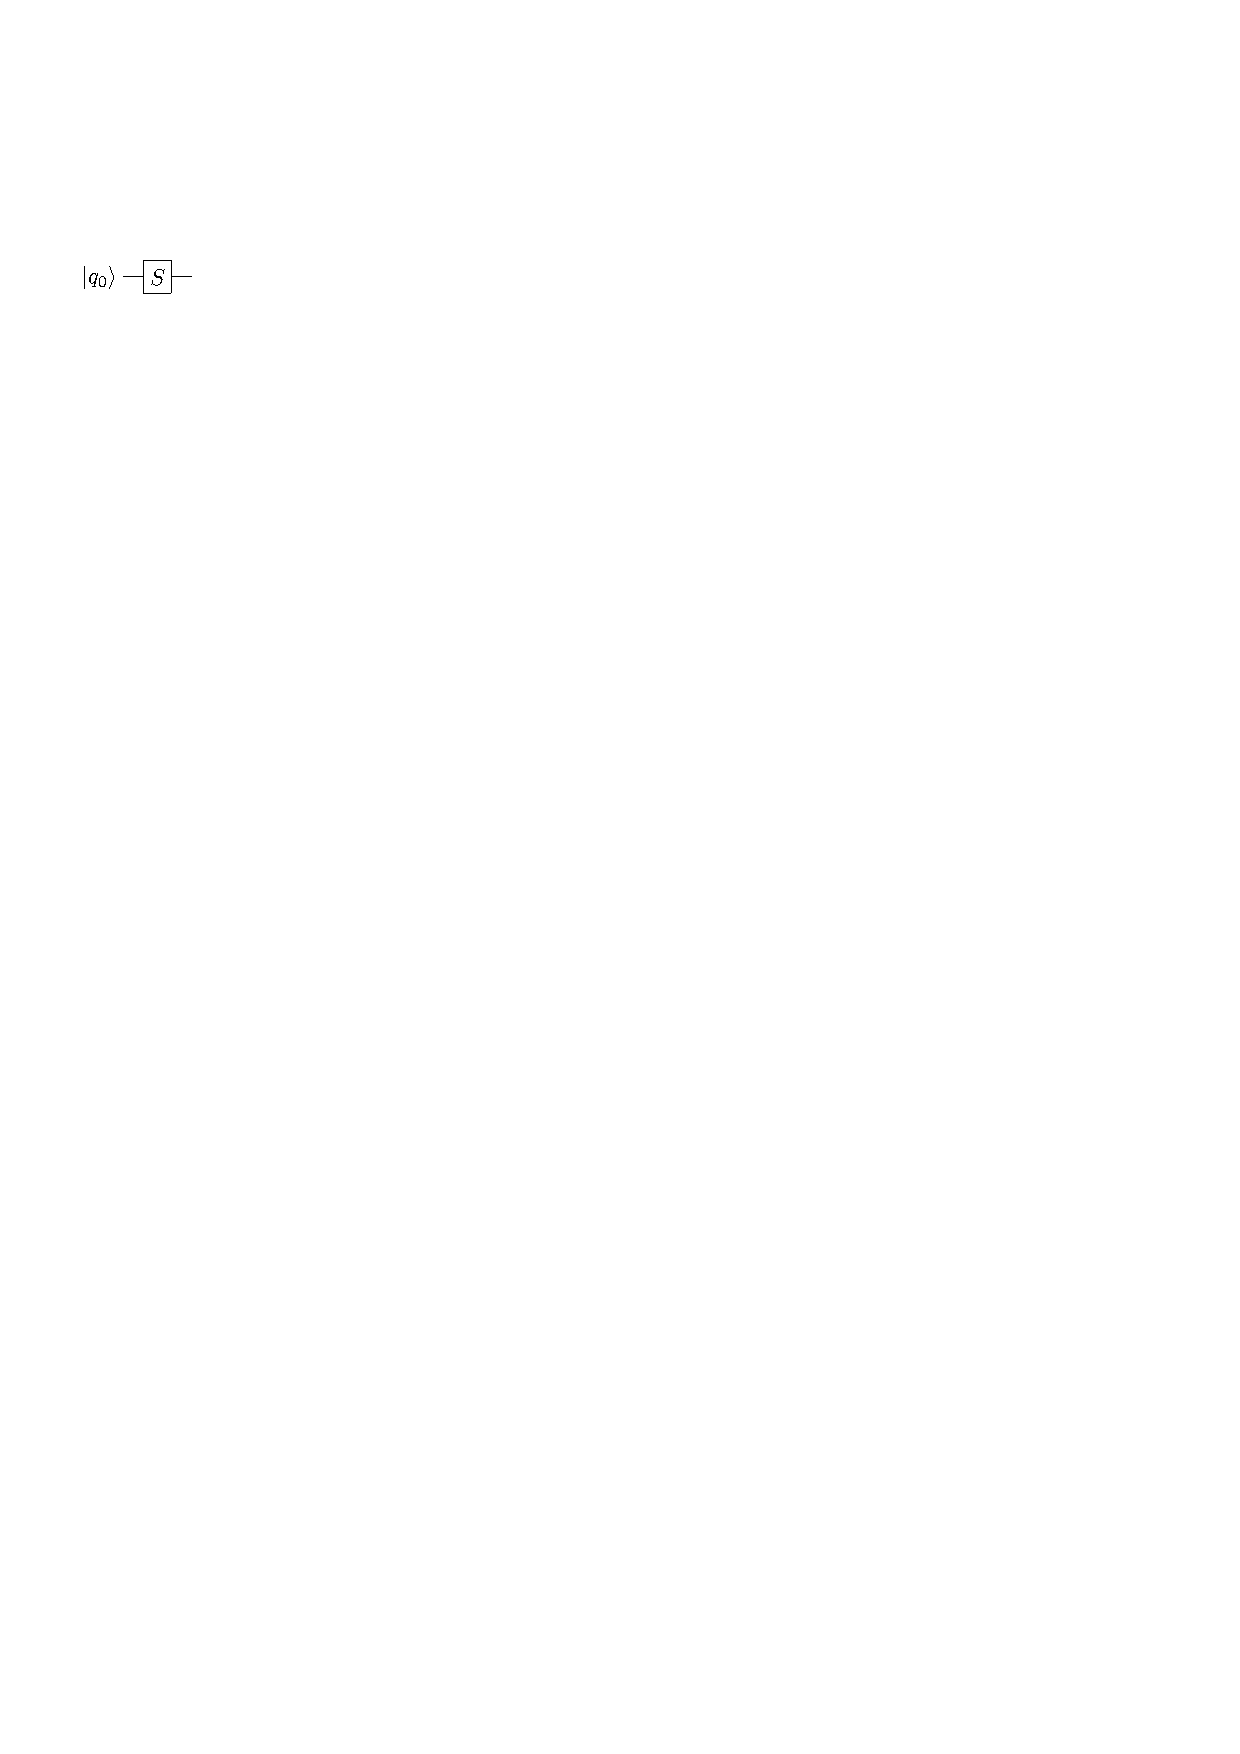
\includegraphics[width=0.1\textwidth]{img/scircuit.png} & $\begin{pmatrix}
 1 & 0 \\ 
 0 & i
 \end{pmatrix}$ & $\sqrt{Z}$ & $\frac{\pi}{2}$ rotation around $\hat{z}$ &  \includegraphics[width=0.2\textwidth]{img/blochsgate.png}\\\midrule
S$^\dagger$ & $-\frac{\pi}{2}$ rotation gate & \includegraphics[width=0.1\textwidth]{img/sdcircuit.png} &  $\begin{pmatrix}
 1 & 0 \\ 
 0 & -i
 \end{pmatrix}$ & Adjoint of S & $-\frac{\pi}{2}$ rotation around $\hat{z}$ & \\\midrule
T & $\frac{\pi}{4}$ rotation gate & \includegraphics[width=0.1\textwidth]{img/tcircuit.png} & $\begin{pmatrix}
 1 & 0 \\ 
 0 & e^{\frac{i\pi}{4}}
 \end{pmatrix}$ & $\sqrt{S}$ & $\frac{\pi}{4}$ rotation around $\hat{z}$ & \includegraphics[width=0.2\textwidth]{img/blochtgate.png}\\\midrule
T$^\dagger$ & $-\frac{\pi}{4}$ rotation gate & \includegraphics[width=0.1\textwidth]{img/tdcircuit.png} & $\begin{pmatrix}
 1 & 0 \\ 
 0 & e^{-\frac{i\pi}{4}}
 \end{pmatrix}$ & Adjoint of T & $-\frac{\pi}{4}$ rotation around $\hat{z}$ & \\\midrule
ZM & Z-basis measurement & 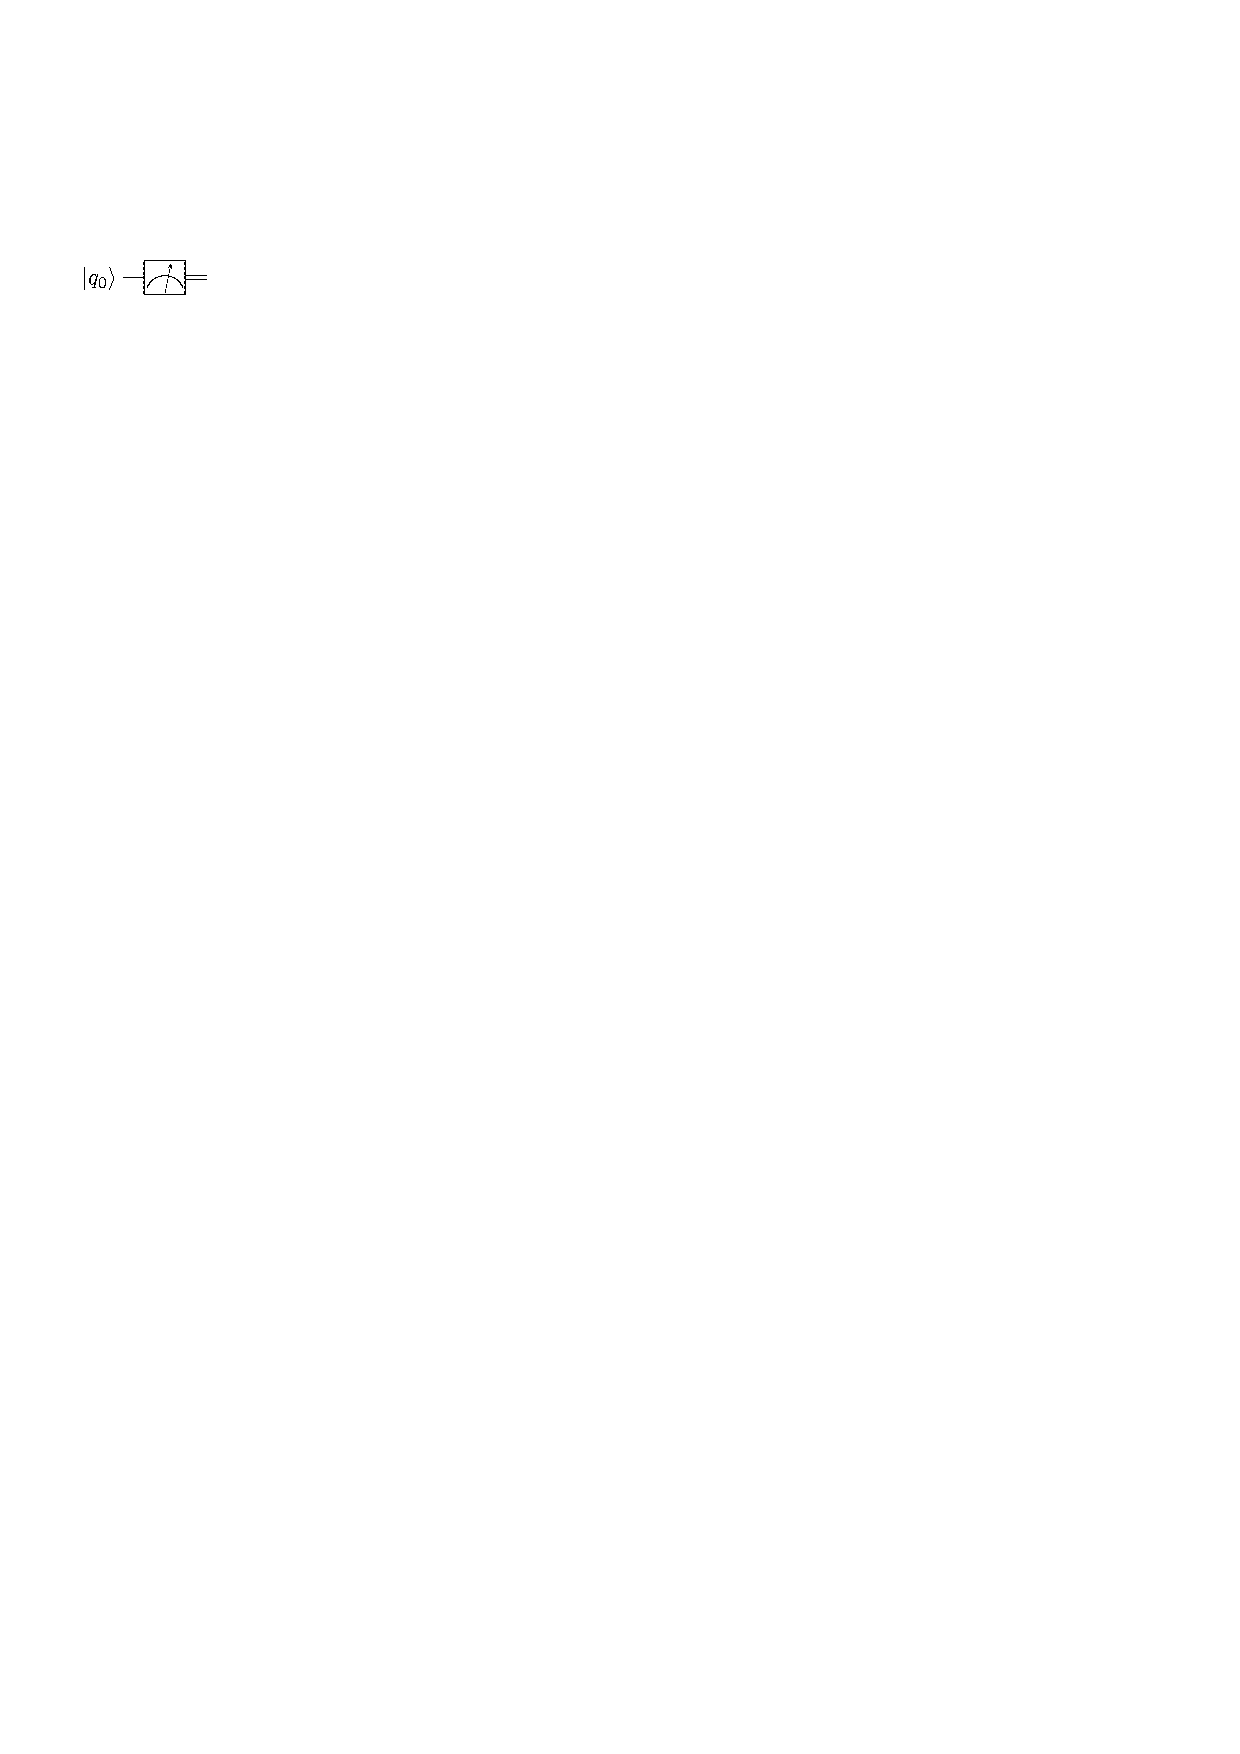
\includegraphics[width=0.1\textwidth]{img/measurecircuit.png} & - & Measurement in standard basis & Collapses the state & - \\
%\midrule
%BM & Bloch measurement & \includegraphics[width=0.1\textwidth]{img/identitycircuit.png} & - & Quantum state tomography & Collapses the state  & -\\
\end{tabular}
\end{table}


%%%%% SUBSECTION: MULTIPLE Q LOGIC GATES


\subsection{Multiple Qubit Gates}
\label{subsubsec:multiqubitgates}

\subsubsection{Controlled NOT Gate}
\label{subsubsubsec:cnotgate}

The most important two-qubit quantum gate is the controlled NOT or CNOT gate given by the following 4x4 matrix:
\begin{equation}
CNOT = \begin{pmatrix}
 \mathbb{1} & 0 \\ 
 0 & X
 \end{pmatrix} = \begin{pmatrix}
 1 & 0 & 0 & 0 \\ 
 0 & 1 & 0 & 0 \\
 0 & 0 & 0 & 1 \\
 0 & 0 & 1 & 0 \\
 \end{pmatrix}
\end{equation}

The CNOT gate takes two qubits, a control and a target qubit, as input. If and only if the control qubit is in the \1 state, the NOT (X) gate is applied to the target qubit. In equations, the CNOT will always be followed by parantheses containing the control (c) qubit followed by the target (t) qubit: CNOT(c,t). The input-output relation (truth table) for the CNOT gate is given in Table~\ref{tab:cnottruthtable} below.

\begin{table}[H]
\begin{center}
\caption{CNOT truth table with first qubit as control, second qubit as target.}\vspace{1ex}
\label{tab:cnottruthtable}
\begin{tabular}{llccc}\hline
Input & Output \\ \hline
00 & 00 \\
01 & 01 \\
10 & 11 \\
11 & 10 \\ \hline
\end{tabular}
\end{center}
\end{table}

To demonstrate the usefulness of the CNOT gate consider starting with two unentangled qubits both in the \0 state,

\begin{equation}
\ket{\phi} = \ket{0} \otimes \ket{0} = \ket{00}
\end{equation}

Applying the H gate onto the first qubit yields the following (still unentangled) state:

\begin{equation}
(H \otimes \mathbb{1}) \ket{\phi} = (H \otimes \mathbb{1}) \ket{00} = \frac{1}{\sqrt{2}} \ket{00} + \frac{1}{\sqrt{2}} \ket{10} 
\end{equation}

Now consider applying the CNOT to this state whereby the control qubit is coloured \textcolor{red}{red} and the target qubit \textcolor{green}{green}.

\begin{equation}
\label{equ:cnotexamples}
CNOT(\textcolor{red}{0},\textcolor{green}{1}) \otimes (\frac{1}{\sqrt{2}} \ket{\textcolor{red}{0}\textcolor{green}{0}} + \frac{1}{\sqrt{2}} \ket{\textcolor{red}{1}\textcolor{green}{0}}) = \frac{1}{\sqrt{2}} \ket{\textcolor{red}{0}\textcolor{green}{0}} + \frac{1}{\sqrt{2}} (\mathbb{1} \otimes X) \ket{\textcolor{red}{1}\textcolor{green}{0}} = \frac{1}{\sqrt{2}} \ket{\textcolor{red}{0}\textcolor{green}{0}} + \frac{1}{\sqrt{2}} \ket{\textcolor{red}{1}\textcolor{green}{1}}
\end{equation}

The last expression in Equ.~\ref{equ:cnotexamples} was used as an example (Equ.~\ref{equ:2qubitnonfactorized}) for entanglement in Section~\ref{subsec:multiplequbitsystems} and it is one of the famous Bell states which are a set of four maximally entangled states (CITATION). Thus, this example demonstrates how the CNOT gate is crucial for the generation of entangled states since it applies the X gate to a qubit depending on the state of a second qubit.

The three most important multi qubit quantum gates CNOT, Toffoli and nCNOT are characterised in Table~\ref{tab:multiqubitgates}.

\begin{table}[H]
\caption{Table of major multi-qubit quantum logic gates where $c_j$ stands for the j\textsuperscript{th} control qubit and $\mathbb{1}_k$ for the kxk identity matrix.}\vspace{1em}
\label{tab:multiqubitgates}
\begin{tabular}{ c  C{1.8cm}  C{2cm}  c C{3cm}}\hline
Gate & Name & Circuit representation & Matrix & Description \\ \midrule
CNOT & Controlled NOT & \includegraphics[width=0.1\textwidth]{img/cnotcircuit.png} & $\begin{pmatrix}
 \mathbb{1} & 0 \\ 
 0 & X
 \end{pmatrix} = \begin{pmatrix}
 1 & 0 & 0 & 0 \\ 
 0 & 1 & 0 & 0 \\
 0 & 0 & 0 & 1 \\
 0 & 0 & 1 & 0 \\
 \end{pmatrix}$ & CNOT($c_1$, target) \\\midrule
Toffoli & Controlled controlled NOT & \includegraphics[width=0.1\textwidth]{img/ccnotcircuit.png}  & $\begin{pmatrix}
 \mathbb{1}_6 & 0 \\ 
 0 & X
 \end{pmatrix} = \begin{pmatrix}
 1 & 0 & 0 & 0 & 0 & 0 & 0 & 0 \\ 
 0 & 1 & 0 & 0 & 0 & 0 & 0 & 0 \\ 
 0 & 0 & 1 & 0 & 0 & 0 & 0 & 0 \\ 
 0 & 0 & 0 & 1 & 0 & 0 & 0 & 0 \\ 
 0 & 0 & 0 & 0 & 1 & 0 & 0 & 0 \\ 
 0 & 0 & 0 & 0 & 0 & 1 & 0 & 0 \\
 0 & 0 & 0 & 0 & 0 & 0 & 0 & 1 \\ 
 0 & 0 & 0 & 0 & 0 & 0 & 1 & 0 \\ 
 \end{pmatrix}$ & CCNOT($c_1$, $c_2$, target)\\\midrule
nCNOT & n-controlled NOT & -  & $\begin{pmatrix}
 \mathbb{1}_{2^n-2} & 0 \\ 
 0 & X
 \end{pmatrix}$ & nCNOT($c_1$,..,$c_n$, target) \\\midrule

\end{tabular}
\end{table}

%%%%% SECTION: MACHINE LEARNING

\section{Classical Machine Learning}
\label{subsec:classicalmachinelearning}

Machine learning can be subdivided into three major fields.

\begin{redbox}
Supervised ML\\
- Based on \emph{input} and \emph{output} data\\
"I know how to classify this data but I need the algorithm to do the computations for me."
\end{redbox}
\begin{greenbox}
Unsupervised ML\\
- Based on \emph{input} data only\\
"I have no clue how to classify this data, can the algorithm create a classifier for me?"
\end{greenbox}
\begin{bluebox}
Reinforcement learning\\
- Based on \emph{input} data only\\
"I have no clue how to classify this data, can the algorithm classify this data and I'll give it a reward if it's correct or I'll punish it if it's not."
\end{bluebox}

This thesis is focussing on quantum-enhancements in the field of supervised machine learning only.

\subsection{k-nearest Neighbour Algorithm}
\label{subsubsec:knearestneighbour}

Understanding the quantum version of the distance weighted $k$-nearest neighbour (kNN) algorithm as described in \cite{Schuld2014} requires prior knowledge of the classical version of the algorithm that will be introduced in this subsection.

Imagine working for a search engine company and you are given the task of classifying unknown pictures of fruits as either apples or bananas. To train your classification algorithm you are given 5 different pictures of apples and 5 different pictures of bananas and will be called the \emph{training data set} ${D}_{T}$. The pictures in ${D}_{T}$ may be taken from different angles, in varying light settings and include different coloured apples and bananas. Two examples of such pictures are shown in Fig.~\ref{img:appleandbanana}. 

\begin{figure}[H]
  \begin{minipage}[t]{0.48\textwidth}
    \includegraphics[width = \textwidth]{img/apple.jpg}
  \end{minipage}
  \hfill
  \begin{minipage}[t]{0.48\textwidth}
    \includegraphics[width = \textwidth]{img/banana.png}
  \end{minipage}
  \caption{Pictures of apple and banana from training data set.\textsuperscript{3}}
  \label{img:appleandbanana}
\end{figure}

\footnotetext[3]{Reprinted from Pixabay, Retrieved December 24, 2016, from \url{https://pixabay.com/en/apple-red-fruit-frisch-vitamins-1632016/} and \url{https://pixabay.com/en/banana-fruit-yellow-1504956/}. Creative Commons Licence 2016 by Pixabay. Reprinted with permission.}

Most of the time, using the full pixel representation of each picture for classification does not lead to optimal results. Therefore, the next step is to select a certain number of characteristic \emph{features} extracted from the pictures in the training set that can be used to differentiate apples from bananas. Such features might be the RGB value of the most frequent pixel colour since bananas and apples have different colour spectra or a measure of the curvature of the main object in the picture since an apple is almost spherical whereas a banana looks more like a bend line. Through the selection \& extraction of features the dimension of the training data set is drastically reduced from a few thousand pixels to a handful of features. The $m$ extracted features for the j\textsuperscript{th} picture are stored in the $m$-dimensional \emph{feature vector} ${v}_{j}$.

Mathematically, the training data set ${D}_{T}$ consists of ten feature vectors ${v}_{0}, {v}_{1},..,{v}_{10}$ that are each assigned to either class $A$ (apple) or $B$ (banana). The training vectors are visualized as yellow and purple circles in Fig.~\ref{fig:knnconcept}.

The kNN algorithm is a non-parametric classifier that given a new unclassified input vector $x$ (red star in Fig.~\ref{fig:knnconcept}) considers the $k$ nearest neighbours within the training set (using a predefined measure of distance) and classifies $x$, based on a majority vote, as either $A$ or $B$. Thereby, $k$ is a positive integer, usually chosen to be small and its value determines the classification outcome. Namely, in the case $k = 3$ in Fig.~\ref{fig:knnconcept}, vector $x$ will be classified as class B (purple) but in the case $k = 6$ it will be labelled class A (yellow).

\begin{figure}[H]
      \centering
       \includegraphics[scale=0.55]{img/knn-concept.png}
       \caption[caption for kNN]{\label{fig:knnconcept} Visualization of a kNN classifier\footnotemark[4]}
\end{figure}

\footnotetext[4]{Reprinted from GitHub, Burton de Wilde, Retrieved September 13, 2016, from \url{http://bdewilde.github.io/blog/blogger/2012/10/26/classification-of-hand-written-digits-3/}. Copyright 2012 by Burton de Wilde. Reprinted with permission.}

In the case of $k = 10$, $x$ would simply be assigned to the class with the most members. In this case, the training vectors should be given distance-dependent weights (such as $\frac{1}{distance}$) to increase the influence of closer vectors over more distant ones.

\chapter{Methods}\label{sec:methods}

All the calculations and plots for this thesis are done in the programming language Python which has a very intuitive syntax and comes with large libraries for scientific computing and plotting.

For the implementation of the quantum kNN algorithm there are two fundamentally different ways: Running it 1) by simulating a QC or 2) by actually executing it on a real QC. The required tools for both possibilities will be explained in the following subsections.

\section{Liqui$\ket{}$}
\label{subsec:simulation}

Classical computers can be used to simulate the behaviour of small quantum computers. Such simulations are associated with exponential computational costs thereby limiting the number of simulated qubits. Since current state-of-the-art quantum technology uses around ten qubits, a classical computer can still be used for simulation.

For the quantum computing simulations in this thesis the quantum simulation toolsuite Liqui$\ket{}$ developed by Microsoft Research will be used. Liqui$\ket{}$ is based on the functional programming language F\# and allows for simulation of up to 30 qubits (verify and cite!). It comes with a large palette of predefined single and multi quantum logic gates and allows for custom-defined quantum gates such as nCNOT and rotation gates controlled by $n$ qubits which is crucial for some of the work done in this thesis.

\begin{figure}[H]
      \centering
       \includegraphics[scale=0.55]{img/liquidcodesnippet.png}
       \caption{\label{fig:liquidsnippet} F\# code snippet from Microsoft's quantum simulation toolsuite Liqui$\ket{}$}
\end{figure}

\section{IBM Quantum Experience}
\label{subsec:ibmqc}

IBM QASM

Earlier this year IBM has enabled public cloud access to their experimental quantum processor containing five non error-corrected superconducting qubits located at the Watson Research Center in New York (VERIFY AND CITATION). Instead of only simulating on classical hardware, this opens up the possibility of executing the QML algorithm on actual quantum hardware.

The so-called IBM Quantum Experience provides the user with access to the "Quantum Composer" which is the main tool for algorithm design. The quantum composer shown in Fig.~\ref{????} consists of 5 horizontal lines, one for each qubit, and enables the user to choose from a universal gate set consisting of 10 quantum logic gates (VERIFY!). Additionally, there are two different measurement types: a) A measurement in the standard z-basis ($\ket{0}$ / $\ket{1}$) resulting in a probability distribution over all possible states and b) a Bloch measurement that visually projects the state onto the Bloch sphere. The user can compose an algorithm by applying up to 40 quantum logic and measurement gates to the five qubits by means of drag-and-drop.

By spending limited user coins the gate sequence of a composed algorithm is then send to IBM's QC in New York and depending on the waiting queue and the availability of the QC the results will be sent back via mail within a few minutes or days. IBM Quantum Experience also allows for free quantum simulations under ideal or real conditions which provides a great tool for experimentation without spending user coins.

The main limitation of the IBM Quantum Experience are the qubit decoherence times since they restrict the maximum number of possible operations before the qubits lose their quantum behaviour and their quantum information. Thus, the number of quantum gates is currently limited to only 40 which essentially means 39 logic gates and 1 measurement gate. The amplitude damping times of the five qubits range from \SI{49.5}{\micro\second} to \SI{85.3}{\micro\second}. Furthermore, the phase damping times range from \SI{56.0}{\micro\second} to \SI{139.7}{\micro\second}. The implementation of a single qubit quantum logic gate takes 130ns and applying a CNOT gate takes 500ns. CITATIONS FOR ALL THESE NUMBERS!

